\chapter[SCP-156 重生石榴]{
    SCP-156 Reanimating Pomegranate \\
    SCP-156 重生石榴
}

\label{chap:SCP-156}

\begin{figure}[H]
    \centering
    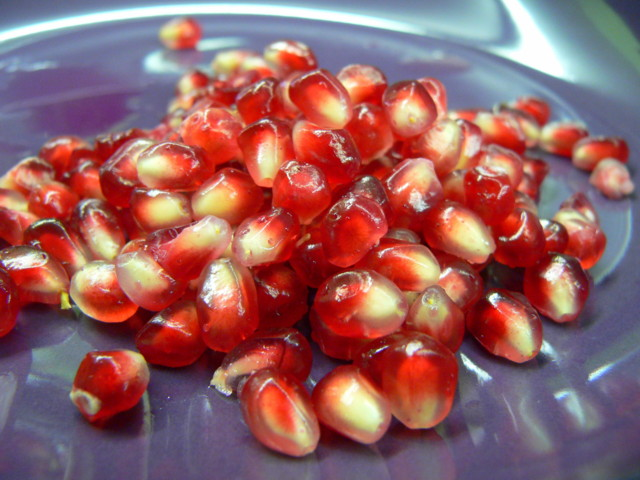
\includegraphics[width=0.5\linewidth]{images/SCP-156.jpg}
    \caption*{一部分SCP-156}
\end{figure}

\bb{项目编号:}SCP-156

\bb{项目等级:}Euclid

\bb{特殊收容措施:}非研究情况下SCP-156都被锁在冷冻储藏单元19c中。每次试验之前和之后都应进行一次检数以确保SCP-156的181个样本数量完整。被影响的对象应出于他们自身的安全而被限制行动并监控。摄入SCP-156者的尸体应被保存于一个带有过滤通风器的保险冷藏间中。所有储藏设施都应被安保摄像头监控。分配给SCP-156的D级人员的处决和尸检应被推迟至他们所涉及的实验结束时那年的三月21日之后。除了进行实验用的D级人员,禁止任何人员食用SCP-156。

\bb{描述:}SCP-156是一堆共181颗石榴籽。籽的数量是恒定的——即,当一个被摄入,或者被一种使其不能被食用的方式摧毁,另外一颗籽会在互相接触的最大的一堆籽中出现。除此之外,石榴籽可以被自由移动。在离开籽堆后(例如一颗籽没有接触到任何其他籽),这颗籽通常在另外一颗新籽进入籽堆之前自行损坏。当被全部分离至任一颗籽都没有接触到另外一颗籽时,一颗被摧毁的籽会随机地与另一颗籽一起出现。当所有籽被同时摧毁时,所有的籽会随机在某颗被摧毁的籽的位置出现。所有重新出现的籽都在旧籽被摧毁的同时以高速摄像机都无法测量更遑论人眼能够捕捉的间隔时间内直接出现,尽管大多数时候观察者都没能注意到新籽直到它们重现的数秒之后。

如果SCP-156被摄入,摄入对象将会继续正常生活直到当年秋分日的中午,那时对象将会暴卒,失去生命体征。尽管在严格意义上死亡了,尸检无法发现死者的死亡原因。除了任何死前就已经存在的情况对象看起来是完全健康的。虽然“死”了,对象不会显示任何腐烂或被分解的状况。摄入对象会持续死亡状态直到下一年的春分中午,届时所有生命体征都会重新激活,即使在死亡期间身体受到严重伤害或被解体至完全失去功能。复活后的医学检查会与在十月21日之前的检查得出完全相同的结果,除了████和█████经常有瘀伤或者覆盖着通常为因用力过度或承受酷刑而产生的疤痕。经过询问,复活的对象可以模糊地回忆起一张苍白的白人男子的脸和一棵枯萎的石榴树。

摄入者将持续每年死而复生直到因为其他原因而死。只有因为摄入SCP-156导致的死亡可以复活。

经历了死而复生的循环的摄入对象会对他们的暂时死亡产生不合常理的恐惧,但是无法解释为什么,确切地说,他们就是害怕。同时,对象会比之前变得更具宿命论。此外对象会出现偏执症,并且会回避任何会对他们造成潜在伤害的物体,包括基金会人员。在经过多次死亡并复生的循环之后,症状会越发严重,并且标示复生的疤痕和瘀伤也会越来越严重直到最终开始包括穿刺性伤口。经过几年后,对象会产生对枯死的植物以及狗的偏执性多疑。摄入之后的第四年到第六年期间对象将不再重生他们的眼睛,并且在复生之后眼睛会继续腐烂。最终,重生后的对象会处于失魂昏迷状态。到达此状态之后对象的死亡并复生仍然继续。

19██年9月21日在希腊████████发生了██人毫无原因的死亡(远远高于一个仅有不到4000人的城镇的自然死亡率)事故之后,SCP-156受到了基金会的注意。然而,直到数个据报告已死者被目击之后(值得注意的是死者本来都被火化)基金会才涉入了此事。经调查死者间唯一的共同点是一起参加了一个家庭聚会。在对有问题的房屋进行了一次标准调查之后,在一个属于已故的A█████ G█████的碗里发现了SCP-156。房屋的剩余部分已经因为所有者表面上的死亡而失修,然而石榴籽仍然保持新鲜。石榴籽被没收用于测试。19██年八月██开始在D级人员身上进行实验。第一个受试者D-E15624死于19██年九月2█,并被解剖验尸。没能发现死因。对象在监视下保持存储。19██年三月2█,对象开始出现脑部活动并且本已在检查中从胸腔中移除的心脏也开始跳动。对象只恢复知觉数秒,在因缺氧陷入昏迷前对象发出了尖叫。D-E15624在之后很快死亡。石榴籽被确认为SCP并且下令进行了长期测试。
